% Options for packages loaded elsewhere
\PassOptionsToPackage{unicode}{hyperref}
\PassOptionsToPackage{hyphens}{url}
%
\documentclass[
]{article}
\usepackage{lmodern}
\usepackage{amssymb,amsmath}
\usepackage{ifxetex,ifluatex}
\ifnum 0\ifxetex 1\fi\ifluatex 1\fi=0 % if pdftex
  \usepackage[T1]{fontenc}
  \usepackage[utf8]{inputenc}
  \usepackage{textcomp} % provide euro and other symbols
\else % if luatex or xetex
  \usepackage{unicode-math}
  \defaultfontfeatures{Scale=MatchLowercase}
  \defaultfontfeatures[\rmfamily]{Ligatures=TeX,Scale=1}
\fi
% Use upquote if available, for straight quotes in verbatim environments
\IfFileExists{upquote.sty}{\usepackage{upquote}}{}
\IfFileExists{microtype.sty}{% use microtype if available
  \usepackage[]{microtype}
  \UseMicrotypeSet[protrusion]{basicmath} % disable protrusion for tt fonts
}{}
\makeatletter
\@ifundefined{KOMAClassName}{% if non-KOMA class
  \IfFileExists{parskip.sty}{%
    \usepackage{parskip}
  }{% else
    \setlength{\parindent}{0pt}
    \setlength{\parskip}{6pt plus 2pt minus 1pt}}
}{% if KOMA class
  \KOMAoptions{parskip=half}}
\makeatother
\usepackage{xcolor}
\IfFileExists{xurl.sty}{\usepackage{xurl}}{} % add URL line breaks if available
\IfFileExists{bookmark.sty}{\usepackage{bookmark}}{\usepackage{hyperref}}
\hypersetup{
  pdftitle={Assignment 4 ETC5513},
  pdfauthor={Yan Ma, Yiwen Zhang, Yuqi Wang, Putu Wahyu Saputra},
  hidelinks,
  pdfcreator={LaTeX via pandoc}}
\urlstyle{same} % disable monospaced font for URLs
\usepackage[margin=1in]{geometry}
\usepackage{longtable,booktabs}
% Correct order of tables after \paragraph or \subparagraph
\usepackage{etoolbox}
\makeatletter
\patchcmd\longtable{\par}{\if@noskipsec\mbox{}\fi\par}{}{}
\makeatother
% Allow footnotes in longtable head/foot
\IfFileExists{footnotehyper.sty}{\usepackage{footnotehyper}}{\usepackage{footnote}}
\makesavenoteenv{longtable}
\usepackage{graphicx,grffile}
\makeatletter
\def\maxwidth{\ifdim\Gin@nat@width>\linewidth\linewidth\else\Gin@nat@width\fi}
\def\maxheight{\ifdim\Gin@nat@height>\textheight\textheight\else\Gin@nat@height\fi}
\makeatother
% Scale images if necessary, so that they will not overflow the page
% margins by default, and it is still possible to overwrite the defaults
% using explicit options in \includegraphics[width, height, ...]{}
\setkeys{Gin}{width=\maxwidth,height=\maxheight,keepaspectratio}
% Set default figure placement to htbp
\makeatletter
\def\fps@figure{htbp}
\makeatother
\setlength{\emergencystretch}{3em} % prevent overfull lines
\providecommand{\tightlist}{%
  \setlength{\itemsep}{0pt}\setlength{\parskip}{0pt}}
\setcounter{secnumdepth}{5}
\usepackage{titling}
\pretitle{\begin{center} 
\includegraphics[width=5in,height=6in]{Images/sam-albury-oA7MMRxTVzo-unsplash.jpg}\LARGE\\}
\posttitle{\end{center}}
\usepackage{fontawesome}
\usepackage[most]{tcolorbox}
\usepackage{xcolor}
\usepackage{sectsty}
\sectionfont{\color{blue}}
\usepackage{verbatim}
\usepackage{fancyhdr}
\pagestyle{fancy}
\usepackage{booktabs}
\usepackage{longtable}
\usepackage{array}
\usepackage{multirow}
\usepackage{wrapfig}
\usepackage{float}
\usepackage{colortbl}
\usepackage{pdflscape}
\usepackage{tabu}
\usepackage{threeparttable}
\usepackage{threeparttablex}
\usepackage[normalem]{ulem}
\usepackage{makecell}
\usepackage{xcolor}
\usepackage[]{natbib}
\bibliographystyle{plainnat}

\title{Assignment 4 ETC5513}
\usepackage{etoolbox}
\makeatletter
\providecommand{\subtitle}[1]{% add subtitle to \maketitle
  \apptocmd{\@title}{\par {\large #1 \par}}{}{}
}
\makeatother
\subtitle{Team name}
\author{Yan Ma, Yiwen Zhang, Yuqi Wang, Putu Wahyu Saputra}
\date{}

\begin{document}
\maketitle

{
\setcounter{tocdepth}{2}
\tableofcontents
}
\clearpage

\hypertarget{introduction}{%
\section{Introduction}\label{introduction}}

Storm can disturb the surface of earth by thunderstorm, snowstorm, rainstorm, sandstorm, flood and so on to cause the road impassibility, the damage of properties and even the injuries and death. Current research shows that hurricanes in the eastern North Pacific can provide water to parts of the southwestern United States and parts of Mexico. More than half of Japan's rainfall comes from typhoons, but at the same time strong convective weather such as hail can also damage buildings and cars parked on the road. , And seriously affected the output of crops such as corn and wheat. This report will focus on the storms happened in America from 2017 to 2019 to analyse it from locations, damages and frequency.

\hypertarget{data}{%
\section{Data}\label{data}}

\hypertarget{data-source}{%
\subsection{Data source}\label{data-source}}

We download the dataset from Storm Events Database data set which contains 31 variables and 187139 observations in total from NOAA \url{https://www.ncdc.noaa.gov/stormevents/}.

\hypertarget{data-limitation}{%
\subsection{Data limitation}\label{data-limitation}}

One of the defects of this dataset is that there is no further division of the scale of disasters, because the losses, casualties and even distribution areas caused by disasters of different scales are different, for example, it is quite difficult to distinguish between small versus large hail through this dataset. So, if there is a further division of the scale of disasters, it will be more conducive to analysis.

\hypertarget{methodology}{%
\section{Methodology}\label{methodology}}

\begin{itemize}
\item
  This project is a descriptive research aiming at virualising and analysing the storms and other significant weather phenomena.
\item
  Use \citet{lubridate} package to covert the date and time columns to proper format.
\item
  Use select function to choose variables for later analysis.
\item
  Use rbind function to bind the data of different years.
\item
  Use \citet{ggplot2} package to create plots.
\end{itemize}

The packages used are as follows :

\begin{itemize}
\item
  ggplot2 \citep{ggplot2}
\item
  lubridate \citep{lubridate}
\item
  readr \citep{readr}
\item
  tidyverse \citep{tidyverse}
\item
  usmap \citep{usmap}
\item
  kableExtra \citep{kableExtra}
\item
  gridExtra \citep{gridExtra}
\item
  bookdown \citep{bookdown}
\item
  plot\_usmap \citep{usmap}
\item
  ggthemes\citep{ggthemes}
\item
  ggmap \citep{ggmap}
\end{itemize}

\clearpage

\hypertarget{section-1}{%
\section{Section 1}\label{section-1}}

From the Table \ref{tab:stormtb} the top 10 numbers of storm events in America are all concentrate in 2017 and 2019 in the past three years. The thunderstorm wind happened most frequently, which is 18617 cases in 2019 and 16472 cases in 2017, after that is hail followed by 10398 in 2017 and 9013 in 2019.

\begin{table}[!h]

\caption{\label{tab:stormtb}Top10 storm events in 3 years }
\centering
\begin{tabular}[t]{l|r|r}
\hline
EVENT\_TYPE & YEAR & count\\
\hline
Thunderstorm Wind & 2019 & 18617\\
\hline
Thunderstorm Wind & 2017 & 16472\\
\hline
Hail & 2017 & 10398\\
\hline
Hail & 2019 & 9013\\
\hline
Flood & 2019 & 4949\\
\hline
Flash Flood & 2019 & 4072\\
\hline
Winter Weather & 2019 & 3803\\
\hline
High Wind & 2019 & 3772\\
\hline
Flash Flood & 2017 & 3662\\
\hline
High Wind & 2017 & 3536\\
\hline
\end{tabular}
\end{table}

Table \ref{tab:countstb} shows the top 10 numbers of storm events happened in America in 2019. first of all is thunderstorm wind happened 18617 times, after that is hail with 9013 cases and flood with 4949 cases and flash flood followed by 4072 cases. The other six are winter weather, high wind, winter storm, heavy snow, marine thunderstorm wind and tornado in order.

\begin{table}[!h]

\caption{\label{tab:countstb}Top5 storm event frequency in 2019}
\centering
\begin{tabular}[t]{l|r}
\hline
EVENT\_TYPE & count\\
\hline
Thunderstorm Wind & 18617\\
\hline
Hail & 9013\\
\hline
Flood & 4949\\
\hline
Flash Flood & 4072\\
\hline
Winter Weather & 3803\\
\hline
\end{tabular}
\end{table}

\clearpage

Figure \ref{fig:locationmap} shows the distributions of the most frequently happened five storm events' locations in 2019. It is clear to see that theses storm events happened more in eastern of America and some in the middle of America.

\begin{figure}

{\centering 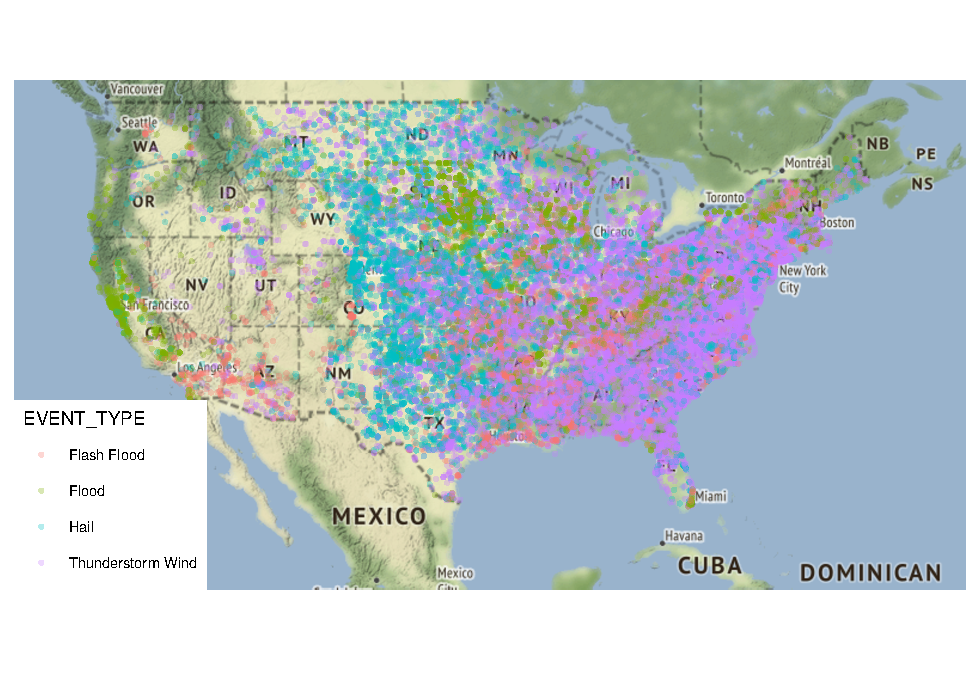
\includegraphics{Images/locationmap-1} 

}

\caption{Top5 storm event locations in 2019}\label{fig:locationmap}
\end{figure}

\clearpage

Figure \ref{fig:TWmonth} shows the thunderstorm wind locations in America in 2019 of different months. It is clear to see that the most active months of thunderstorm wind were from May to August. Furthermore, the locations of theses events happened from middle and east of America slowly transformed to the east from July to October.

\begin{figure}

{\centering 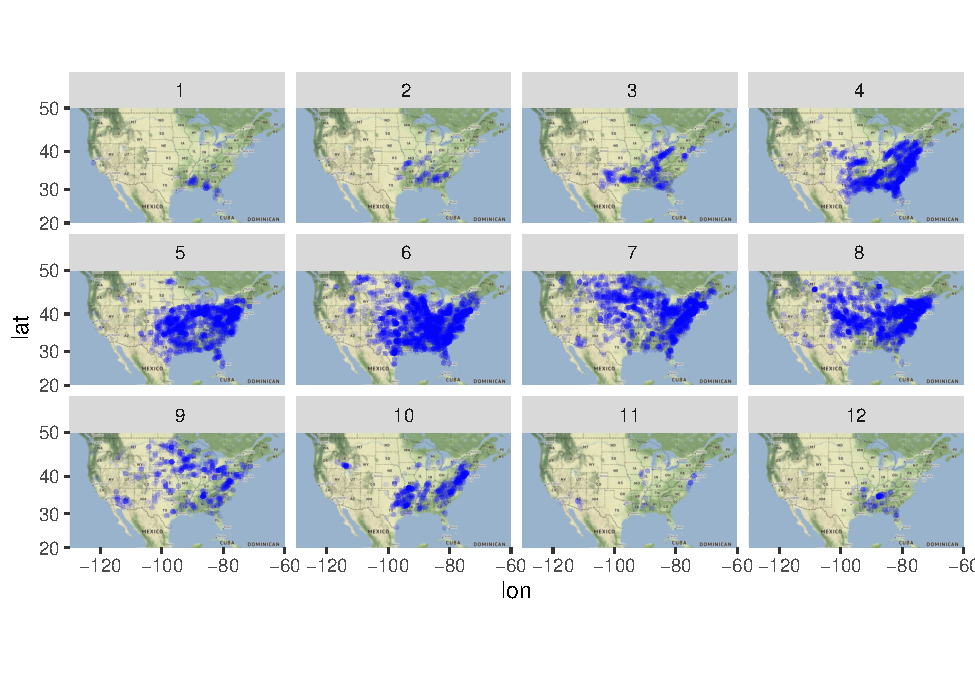
\includegraphics{Images/TWmonth-1} 

}

\caption{Thunderstorm locations by month in 2019}\label{fig:TWmonth}
\end{figure}

\clearpage

Table \ref{tab:statestb} displayed the number of thunderstorm wind happed in different states of America in 2019. As we can see from the table, except for Kansas, Texas and Missouri, the top ten states are all located in the east of America.

\begin{table}[!h]

\caption{\label{tab:statestb}Top10 states by number of thunderstorm in 2019}
\centering
\begin{tabular}[t]{l|r}
\hline
STATE & count\\
\hline
PENNSYLVANIA & 1245\\
\hline
VIRGINIA & 1199\\
\hline
TEXAS & 1047\\
\hline
NEW YORK & 903\\
\hline
OHIO & 891\\
\hline
KANSAS & 848\\
\hline
NORTH CAROLINA & 791\\
\hline
GEORGIA & 673\\
\hline
MISSOURI & 648\\
\hline
SOUTH CAROLINA & 619\\
\hline
\end{tabular}
\end{table}

Figure \ref{fig:monthplot} shows that the number of thunderstorm wind occurred in different states by month. The thunderstorm wind most frequently happened from May to August. However the peak of the number of such cases were different from some states, August is the peak month of some eastern America states like New York, Pennsylvania and Virginia, for the middle of America states like Texas and Missouri, the peak months were May and June.

\begin{figure}

{\centering 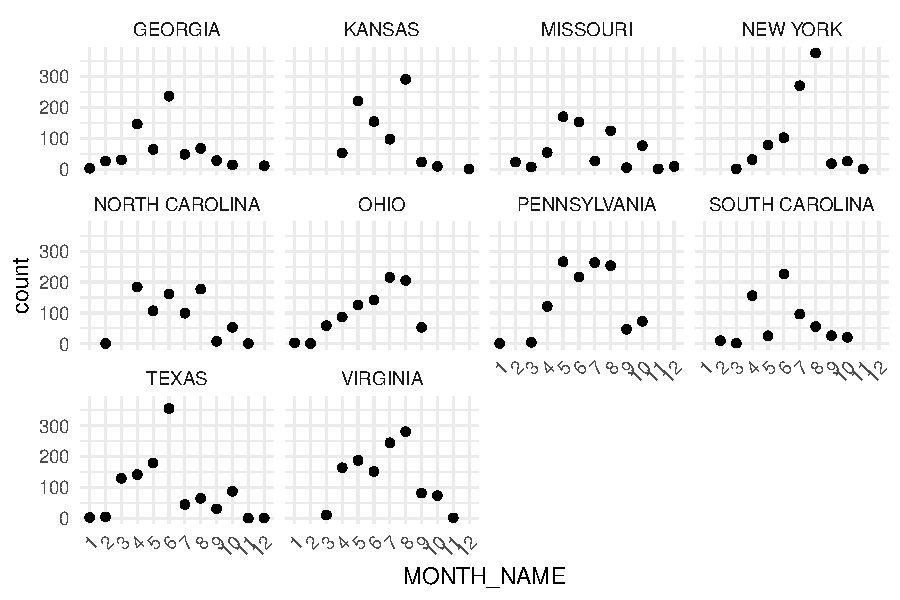
\includegraphics{Images/monthplot-1} 

}

\caption{The nuber of thunderstorm events of top10 states in diffenrent month}\label{fig:monthplot}
\end{figure}

\clearpage

\hypertarget{section-2-injuries-and-deaths}{%
\section{Section 2: Injuries and Deaths}\label{section-2-injuries-and-deaths}}

This section will focus on the injuries and deaths caused by the storm events and other unusual weather phenomena across the US from 2017 to 2019.

\hypertarget{direct-injuries-and-deaths-by-month-and-year}{%
\subsection{Direct injuries and deaths by month and year}\label{direct-injuries-and-deaths-by-month-and-year}}

Figure \ref{fig:fig1} and \ref{fig:fig2} shows the total direct injuries and deaths of the storm events by month.

Over all the years, there are less direct injuries of storm events from September to December, while more direct injuries happened on January June and July. Most direct deaths happened on January, June to September and November.

There are several noticeable time periods. First, there are over 500 injuries and over 200 deaths on July 2018. Second, over 100 deaths happened on November 2018.

\begin{figure}
\centering
\includegraphics{report_files/figure-latex/fig1-1.pdf}
\caption{\label{fig:fig1}Total direct injuries by month}
\end{figure}

\begin{figure}
\centering
\includegraphics{report_files/figure-latex/fig2-1.pdf}
\caption{\label{fig:fig2}Total direct deaths by month}
\end{figure}

\clearpage

\hypertarget{direct-injuries-and-deaths-by-state}{%
\subsection{Direct injuries and deaths by state}\label{direct-injuries-and-deaths-by-state}}

Figure \ref{fig:fig3} shows the direct injuries of each state through 2017 to 2019. In 2017, Georgia had over 150 direct injuries which is the most among all the states. In 2018, California had over 350 direct injuries which is the most among all the states due to a historical largest wildfire(\citet{california}). Meanwhile, Oklahoma and Missouri also had over 200 direct injuries. The most injuries in 2019 happened in Ohio, with over 200 injuries.

\begin{figure}
\centering
\includegraphics{report_files/figure-latex/fig3-1.pdf}
\caption{\label{fig:fig3}Total direct injuries by state}
\end{figure}

\clearpage

Figure \ref{fig:fig4} shows the direct deaths of each state through 2017 to 2019. In 2017, Texas had about 100 direct deaths, which is the most among all the states. In 2018, Arizona had over 150 direct deaths and California had about 150 direct deaths, which are more than other states. In 2019, no state had more than 50 direct deaths, and Texas is slightly higher than others.

\begin{figure}
\centering
\includegraphics{report_files/figure-latex/fig4-1.pdf}
\caption{\label{fig:fig4}Total direct deaths by state}
\end{figure}

\clearpage

\hypertarget{direct-injuries-and-deaths-by-major-event-type}{%
\subsection{Direct injuries and deaths by major event type}\label{direct-injuries-and-deaths-by-major-event-type}}

Table \ref{tab:tab1} shows the top 5 types of events with most direct injuries from 2017 to 2019. And figure \ref{fig:fig5} shows the injuries they caused every year. Tornado caused most direct injuries in 2017 and 2019, while heat caused more direct injuries than other types of events in 2018.

\begin{table}[!h]

\caption{\label{tab:tab1}Major event types cause direct injuries over years}
\centering
\begin{tabular}[t]{lr}
\toprule
EVENT\_TYPE & injury\_event\\
\midrule
\rowcolor{gray!6}  Tornado & 1253\\
Heat & 545\\
\rowcolor{gray!6}  Thunderstorm Wind & 480\\
Excessive Heat & 306\\
\rowcolor{gray!6}  Lightning & 268\\
\bottomrule
\end{tabular}
\end{table}

\begin{figure}
\centering
\includegraphics{report_files/figure-latex/fig5-1.pdf}
\caption{\label{fig:fig5}Total direct injuries by event type}
\end{figure}

\clearpage

Table \ref{tab:tab2} shows the top 5 types of events with most direct deaths from 2017 to 2019. And figure \ref{fig:fig6} shows the deaths they caused every year. Excessive Heat caused most direct deaths among the five major event types in 2018, while flash flood caused slightly more direct deaths in 2017 and 2019. In addition, direct deaths caused by wildfire is decreasing in this time period.

\begin{table}[!h]

\caption{\label{tab:tab2}Major event types cause deaths over years}
\centering
\begin{tabular}[t]{lr}
\toprule
EVENT\_TYPE & death\_event\\
\midrule
\rowcolor{gray!6}  Excessive Heat & 238\\
Flash Flood & 219\\
\rowcolor{gray!6}  Heat & 213\\
Rip Current & 179\\
\rowcolor{gray!6}  Wildfire & 139\\
\bottomrule
\end{tabular}
\end{table}

\begin{figure}
\centering
\includegraphics{report_files/figure-latex/fig6-1.pdf}
\caption{\label{fig:fig6}Total direct deaths by event type}
\end{figure}

\clearpage

\hypertarget{section-3}{%
\section{Section 3}\label{section-3}}

\hypertarget{the-trend-of-occurence-of-the-top-five-most-frequent-events-changing-by-year}{%
\subsection{The trend of occurence of the top five most frequent events changing by year}\label{the-trend-of-occurence-of-the-top-five-most-frequent-events-changing-by-year}}

In this section, the main purpose is to explore the trend of occurence of the top five most frequent events changing by year both across the whole USA and in each state. First, create a table and group the data by ``STATE'' and ``YEAR''. Then count the times of occurence for all events and rename the name of this column as ``FREQ'' to present the frequency. And next, create a new table to arrange the data by descending order with displaying the top 5 events that happen most frequently. Then, use ``right\_join'' to connect these two tables. Finally, create two figures to display the trend of occurence of the top 5 event changing by year.

\begin{table}[!h]

\caption{\label{tab:tablefrequency}The frequency of the events}
\centering
\begin{tabular}[t]{lrlr}
\toprule
STATE & YEAR & EVENT\_TYPE & FREQ\\
\midrule
ALABAMA & 2017 & Coastal Flood & 4\\
ALABAMA & 2017 & Cold/Wind Chill & 1\\
ALABAMA & 2017 & Drought & 92\\
ALABAMA & 2017 & Extreme Cold/Wind Chill & 1\\
ALABAMA & 2017 & Flash Flood & 132\\
\addlinespace
ALABAMA & 2017 & Flood & 24\\
ALABAMA & 2017 & Frost/Freeze & 11\\
ALABAMA & 2017 & Funnel Cloud & 2\\
ALABAMA & 2017 & Hail & 201\\
ALABAMA & 2017 & Heavy Rain & 6\\
\bottomrule
\end{tabular}
\end{table}

\begin{table}[!h]

\caption{\label{tab:tablefrequencynew}Top five most frequent events}
\centering
\begin{tabular}[t]{l}
\toprule
EVENT\_TYPE\\
\midrule
Thunderstorm Wind\\
Hail\\
Flood\\
Flash Flood\\
Winter Weather\\
\bottomrule
\end{tabular}
\end{table}

\begin{table}[!h]

\caption{\label{tab:rightjointable}Occurence of top five most frequent events}
\centering
\begin{tabular}[t]{lrlr}
\toprule
STATE & YEAR & EVENT\_TYPE & FREQ\\
\midrule
ALABAMA & 2017 & Thunderstorm Wind & 630\\
ALABAMA & 2018 & Thunderstorm Wind & 495\\
ALABAMA & 2019 & Thunderstorm Wind & 591\\
ALASKA & 2019 & Thunderstorm Wind & 2\\
ARIZONA & 2017 & Thunderstorm Wind & 116\\
\addlinespace
ARIZONA & 2018 & Thunderstorm Wind & 185\\
ARIZONA & 2019 & Thunderstorm Wind & 97\\
ARKANSAS & 2017 & Thunderstorm Wind & 423\\
ARKANSAS & 2018 & Thunderstorm Wind & 411\\
ARKANSAS & 2019 & Thunderstorm Wind & 359\\
\bottomrule
\end{tabular}
\end{table}

\begin{figure}
\centering
\includegraphics{report_files/figure-latex/frequencyplot-1.pdf}
\caption{\label{fig:frequencyplot}Occurence of top five most frequent events changing by year}
\end{figure}

Table \ref{tab:tablefrequency} displays the first ten lines of the frequency of all events. And Table \ref{tab:tablefrequencynew} displays the top five most frequent events. And Table \ref{tab:rightjointable} displays the first ten lines of the final results of the occurence of top five most frequent events. It can be seen that top 5 events have occurred in some regions in three years for example, thunderstorm wind has occurred in Alabama in three yearsfrom 495 times to 630 times , while it has only occurred twice in Alaska in 2019.
Figure \ref{fig:frequencyplot} presents the occurence of top five most frequent events across the whole USA, we could see that thunderstorm wind showed an increasing trend during three years. And hail showed a slow growth in 2017-2018, followed by a sharp decline in 2018-2019. As for the winter weather, it has been on a downward trend for three years, but the slowdown from 2017 to 2018 was larger than that from 2018 to 2019. What's more, flash flood kept growing, but slowed down between 2018 and 2019. At last, flood kept a slow decline at first, then turned into a significant rise.
We could see that most events have a similar trend, but hail has decreased in 2018 to 2019 years, which is possibly due to increased melting level heights and greater atmospheric instability.\citep{dessensberthetsanchez2015} Correspondingly, the number of floods increased from 2018 to 2019, which is increasingly common due to years of relative sea level increases and El Nino.\citep{floodingdaysin2018}

\clearpage

\hypertarget{section-4}{%
\section{Section 4:}\label{section-4}}

Based on the calculation of the number of tornadoes that occur each year, the United States becomes a country with more than 1000 events each year. \citet{USTornad80} Table \ref{tab:table-tornado} shows the number of tornadoes from 2017 to 2019 in the United States.
The table made by \texttt{kable} function from \texttt{knitr} package. \citet{knitr}

\begin{table}[!h]

\caption{\label{tab:table-tornado}Total number of Tornado that occurs from 2017-2019 in United States}
\centering
\begin{tabular}[t]{r|l|r}
\hline
YEAR & EVENT\_TYPE & n\\
\hline
2017 & Tornado & 1647\\
\hline
2018 & Tornado & 1250\\
\hline
2019 & Tornado & 1728\\
\hline
\end{tabular}
\end{table}

We use \texttt{ggplot2} package to map the distribution overtime. \citet{ggplot2} To see the number of tornadoes that occur each month during these three years can be seen in Figure \ref{total-f-scale}. From this plot, it can be seen that most tornadoes occur on average in the range of April and May. 2019 recorded a high number of tornadoes in May compared to the previous two years.

\begin{figure}
\centering
\includegraphics{report_files/figure-latex/total-f-scale-1.pdf}
\caption{\label{fig:total-f-scale}Tornado frequency from 2017-2019 in USA}
\end{figure}

\clearpage

Figure \ref{fig:map-tornado} shows the map of the United States with the highest number of tornadoes during 2017-2019. The map plotted using \texttt{plot\_usmap} function from \texttt{usmap} package. \citet{usmap}

\begin{figure}
\centering
\includegraphics{report_files/figure-latex/map-tornado-1.pdf}
\caption{\label{fig:map-tornado}United States map of total tornado in each state}
\end{figure}

Each tornado that occurs has a scale. Based on dataset documentation, enhanced Fujita Scale describes the strength of the tornado based on the amount and type of damage caused by the tornado. \citet{documentation}
The F scale listed as Table \ref{tab:scale} :

\begin{table}[!h]

\caption{\label{tab:scale}Level of Tornadoes}
\centering
\begin{tabular}[t]{l|l|l}
\hline
Scale & Category & Speed\\
\hline
EF0 & Light & 40 – 72 mph\\
\hline
EF1 & Moderate & 73 – 112 mph\\
\hline
EF2 & Significant & 113 – 157 mph\\
\hline
EF3 & Severe & 158 – 206 mph\\
\hline
EF4 & Devastating & 207 – 260 mph\\
\hline
EF5 & Incredible & 261 – 318 mph\\
\hline
EFU & Unknown & Unknown\\
\hline
\end{tabular}
\end{table}

When there is no tornado damage, but there is evidence a tornado existed (citation)

In Table \ref{tab:tornado-state}, Texas is the state that has been hit the most by Tornadoes---followed by Kansas, Alabama, Missouri, and Minnesota. The top four states have experienced Tornadoes on an EF4 scale from 2017 to 2019. The table style use \texttt{kableExtra} package. \citet{kableExtra}

\begin{table}[!h]

\caption{\label{tab:tornado-state}Tornado frequency by scale for each state in USA from 2017-2019}
\centering
\begin{tabular}[t]{l|r|r|r|r|r|r}
\hline
STATE & EF0 & EF1 & EF2 & EF3 & EF4 & EFU\\
\hline
TEXAS & 201 & 92 & 45 & 13 & 1 & 75\\
\hline
KANSAS & 116 & 41 & 11 & 6 & 1 & 38\\
\hline
ALABAMA & 111 & 86 & 18 & 1 & 1 & NA\\
\hline
MISSOURI & 102 & 98 & 14 & 5 & 1 & 2\\
\hline
MINNESOTA & 101 & 75 & 7 & NA & NA & 1\\
\hline
\end{tabular}
\end{table}

As the state with the highest number of tornadoes, we analyze Texas deeper. Figure \ref{fig:tornado-texas} shows the number of tornadoes that occur overtime based on scale. In general, the number of tornadoes varies each year. EF0 occurs almost every year, but in 2019, the number of EF0 occurs more than 40 times in May. In 2018, the number of tornadoes on the EF1 and EF2 scales was less than in 2017 and 2019. The EF4 happened once in 2018.

\begin{figure}
\centering
\includegraphics{report_files/figure-latex/tornado-texas-1.pdf}
\caption{\label{fig:tornado-texas}Tornado scale per month in Texas}
\end{figure}

Figure \ref{fig:tornado-texas-2019} tells what time of day a tornado with a particular scale occurs in Texas in 2019. Generally, there are differences in each month. May is the most prominent month with almost every day some tornadoes occur.

\begin{figure}
\centering
\includegraphics{report_files/figure-latex/tornado-texas-2019-1.pdf}
\caption{\label{fig:tornado-texas-2019}Tornado by hour distribution that happened in Texas in 2019}
\end{figure}

\clearpage

\hypertarget{conclusion}{%
\section{Conclusion}\label{conclusion}}

\begin{itemize}
\item
  The most active months of thunderstorm wind were from May to August. Furthermore, the locations of theses events happened from middle and east of America slowly transformed to the east from July to October.
\item
  Over all the years, there are less direct injuries of storm events from September to December, while more direct injuries happened on January June and July. Most direct deaths happened on January, June to September and November.
\item
  In 2017, Georgia had the most direct injuries and Texas had the most direct deaths among all the states. In 2018, California had the most direct injuries and Arizona had the most direct deaths among all the states. In 2019, no state had more than 50 direct deaths, and Texas is slightly higher than others while Ohio had the most direct injuries.
\item
  Tornado caused most injuries in 2017 and 2019, while heat caused more injuries than other types of events in 2018. Excessive Heat caused most direct deaths among the five major event types in 2018, while flash flood caused slightly more direct deaths in 2017 and 2019. In addition, direct deaths caused by wildfire is decreasing in this time period.
\item
  Seeing from top five most frequent events, most events have a similar trend. However, hail has decreased in 2018 to 2019 years with floods increasing instead.
\item
  Tornado mostly happen in May while Texas is the state with the highest number of tornado in USA.
  \clearpage
\end{itemize}

  \bibliography{references.bib}

\end{document}
